\documentclass[aps,prb,reprint]{revtex4-1}

\usepackage[dvipdfmx]{graphicx}
\usepackage{graphicx}
\usepackage{bm}
\makeatletter

\begin{document}

\title{Statement of Purpose: Connecting Science in China and Japan}
\author{Nobuyoshi Hiramatsu}
\affiliation{Department of Applied Physics, the University of Tokyo.}
\maketitle

Main purpose of my PhD study at Physics department in Tsinghua University is to acquire knowledge and experiences that enable me connecting Chinese-Japanese communities in Science and Technology. Chinese community has been getting a core of Research and Development (R\&D) in recent years\cite{RD}, and Japanese has been an unique community which supports great researches and economy. Collaborations of these two communities must boost world's knowledge and economy; however, an amount of their collaborations, especially in younger generations, are getting decreased despite their cultural similarity and geometrical proximity. Therefore, my prospective contribution to Japan and China for facilitating collaborations in both science and industrial field, must be significant! 
\vspace{-0.5zh}
\begin{figure}[h]
  \begin{center}
   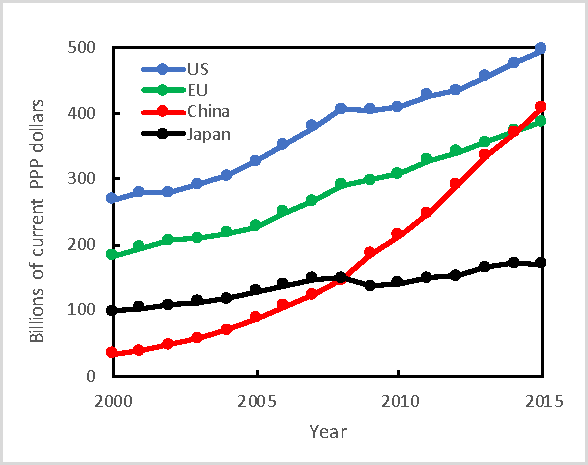
\includegraphics[width=\hsize]{RD.pdf}
  \end{center}
  \vspace{-1zh}
  \caption{Gross domestic expenditures on R\&D: 2000-2015 (PPP: Purchasing Power Parity.)\cite{RD}}
  \label{fig:RD}
\end{figure}

To achieve my goal at Tsinghua, studying in Prof. Yu's Group is the most suitable for several reasons. First, Yu group has great equipments and experiences to develop oxide-films with four PLD systems and an incoming MBE system, as well as equipments for sample-characterization and measurement with XRD, AFM, MFM, Raman spectroscopy, PPMS, and MPMS. Moreover, from my point of view, current focus of Yu Group in manipulation of the functional oxide films using ionic liquid seems unique, and promising for both scientific and application side. In this research environment, I could accumulate my various experiences of oxide-film-physics for PhD study, to be one of my core competences in the future. This experience should be highly beneficial to get a responsible position in Japan or China, to achieve my goal. Second, Dr. Yu is an experienced researcher who acquired his PhD at UC Berkeley in US and did his postdoc at RIKEN in Japan, and he is engaging in many collaborations with researchers in China, US and Japan. I hope I do research in the collaborations, so as to learn how to conduct good research in good international relations and friendships. Finally, Dr. Yu is in a joint position at the Center of Emergent Matter Science, RIKEN in Japan and Physics department at Tsinghua University in China. I hope I could directly help communication for students and faculties in RIKEN and Tsinghua as a Japanese-Chinese speaking PhD student in Yu group.

I prepared enough to contribute to Yu group as a PhD student. I have been awarded my higher education at the department of electronics and controlling science, Toyama National College of Technology for associate degree; and at the department of applied physics, the University of Tokyo for bachelor's degree.  In the university of Tokyo, I measured fundamental properties of the electromagnetic-surface-mode or surface plasmon polaritons on noble metal and publish a paper\cite{paper}, and do experiments of metastable superconductivity. I have experiences to be beneficial at Yu group, including optical experiment, electron-lithography, evacuation, helium transferring, and constructing a low-temperature probe for resistance measurements. Furthermore, I have experienced a practical internship at an analog-semiconductor-sensor manufacturer in Austria. We proposed very small smoke detecting device down to cubic 1mm by using Very Large Scale Integration(VLSI)-technique with Vertical Cavity Surface Emitting Laser (VCSEL), and published a patent\cite{patent}. These educations and experiences will help me to assimilate into the group.

As mentioned, I need opportunities in Prof. Yu's group, to contribute to both Chinese and Japanese society as well as to science in the world.

%\vspace{-1em}
%\renewcommand{\refname}{}
\bibliography{personal_statement_tsinghua}

\end{document}